\documentclass[11pt,a4paper]{article}
\usepackage[margin=23mm]{geometry}
\usepackage[T1]{fontenc}
\usepackage{lmodern}
\usepackage{booktabs}
\usepackage{longtable}
\usepackage{hyperref}
\emergencystretch=2em
\usepackage{tikz}
\usetikzlibrary{positioning,arrows.meta}
\title{Tier 2A/2B: the optional executable-model contract\\
\large a validated declaration facet, and a port axis independent of the sign}
\date{Created-at: 2026-09-06 03:52 +02:00}
\begin{document}
\maketitle

\paragraph{Entry state, measured after fetch.}
Core \texttt{main@4acba44}, clean, \textbf{fully green}: 134 + 254 + 2 + 5 = 395 passed, 0 failed,
7 ignored; \texttt{clippy -p hymeko\_core --all-targets -D warnings} 0; \texttt{fmt --check} 0.
The 2026-09-05 baseline failure \texttt{v1\_corpus\_digest\_is\_unchanged} \textbf{now passes} --- it
was resolved upstream, and that earlier ``not green'' record is superseded. Provider
\texttt{hymeko@1032a2d}. Downstream Nagare witnesses on this core: \texttt{merkle\_digest\_soundness}
14/14 with 0 ignored, \texttt{canonical\_mlp\_witness} 2/2, \texttt{contract\_consumer\_gate} 10/10.

\paragraph{The gap, re-reproduced on this tip.} Of the eleven ownership rows, exactly one is
\texttt{CanonicalOwned} (the semantic model digest, upstream). Rows 2, 4, 7 and 9 are
\texttt{Missing}; 1, 3, 5, 6, 8, 10 are \texttt{CarrierOnly}. Verified by direct inspection: the IR
entity set in \texttt{ir/ir.rs} is unchanged, no \texttt{Role}/\texttt{Shape}/\texttt{DType}/
direction type exists anywhere in \texttt{hymeko\_core/src}, \texttt{ir::coherence} contains no
annotation inspection, and \texttt{tensor/compute/mod.rs:26} still declares \texttt{DType}
deliberately absent.

%======================================================================
\section{The design question that comes first}

\textbf{Most HyMeKo declarations are not tensors or operators.} The tracked corpus describes service
networks, robotics meta-graphs and P-graph structures; the 111 \texttt{.hymeko} fixtures under
\texttt{tests/} contain no neural model. A mandatory \texttt{role}/\texttt{shape}/\texttt{dtype} on
every \texttt{DeclNode} would therefore be wrong on its face: it would force a meaningless answer
onto every existing declaration and move every existing digest.

The contract is consequently an \textbf{optional facet}, not a widening of the universal
declaration:

\begin{center}\small
\begin{tabular}{@{}lp{95mm}@{}}
\toprule
\texttt{DeclNode.model: Option<ModelFacet>} & absent (\texttt{None}) on every declaration that is
not part of an executable model --- which is every declaration in the current corpus \\
\texttt{ModelFacet::Tensor} & \texttt{\{role, shape, dtype\}}: the declaration is a tensor \\
\texttt{ModelFacet::Operator} & \texttt{\{identity\}}: the declaration is a typed operator \\
\bottomrule
\end{tabular}
\end{center}

A document is an \emph{executable model} exactly when at least one declaration carries a facet.
Only then does the completeness validator engage. This is what keeps the general IR general, and it
is the reason the change can be additive rather than a migration.

\paragraph{Annotation tags are not the authority.} Where a facet is present, the typed fields are
authoritative and the tags are decoration. The acceptance gate is adversarial: an executable model
whose tags are replaced by a meaningless word must still validate and still digest identically,
while removing a typed field must fail. That is the inverse of today's
\texttt{core\_accepts\_a\_model\_whose\_tag\_vocabulary\_is\_meaningless}, which currently passes and
must, after 2A, fail for a model that declares facets.

%======================================================================
\section{Compatibility, proven before the first edit}

Three questions decide whether this boundary may proceed at all.

\begin{center}\small
\begin{tabular}{@{}p{34mm}p{104mm}@{}}
\toprule
Question & Evidence gathered at entry \\
\midrule
Do absolute V2 digest goldens exist? & \textbf{No.} \texttt{tests/unified\_ir/verification/semantic\_digest.rs} contains \textbf{zero} 64-hex constants; every assertion is relative (moves / does not move). The only absolute goldens are v1-family: \texttt{KAT\_CORPUS\_DIGEST}, the four \texttt{frozen\_hash.rs} KATs, and the unrelated \texttt{sparse\_workload\_kat}. \textbf{So the algorithm version may be raised, and v1 must not be touched.} \\
Is the CBOR wire serde-derived? & \textbf{Yes} --- \texttt{ciborium::ser::into\_writer(\&payload)} over \texttt{CborPayload}, which already carries an explicit \texttt{schema\_version: u16} that rejects missing and unsupported versions. An additive field with \texttt{\#[serde(default)]} therefore decodes every existing payload unchanged. \\
How many \texttt{RefAtomR} construction sites? & \textbf{Five} literal sites in \texttt{hymeko\_core/src} (\texttt{ir/ir.rs}, \texttt{ir/incidence.rs}, \texttt{resolution/resolve.rs}, \texttt{writers/cbor\_writer/tests.rs}). The 2B inventory is bounded and enumerable before any signature moves. \\
\bottomrule
\end{tabular}
\end{center}

\paragraph{Versioning.} \texttt{SEMANTIC\_DIGEST\_ALGO\_VERSION} $2 \rightarrow 3$, because the
covered set grows. \texttt{canonical\_program\_hash} v1 is \textbf{not touched}: no signature, no
byte, no \texttt{algo\_version}, so \texttt{KAT\_CORPUS\_DIGEST} and the frozen KATs hold unchanged.
The CBOR \texttt{schema\_version} rises only if the encoded shape changes in a way old readers
cannot ignore; the additive-optional form is chosen precisely so it does not.

\paragraph{Legacy digests.} A declaration with \texttt{model: None} contributes one domain-tagged
absence marker. Every V2 digest therefore moves once, at the version bump --- which is sound because
no artifact pins a V2 value --- and never again for a legacy document.

%======================================================================
\section{Architecture}

\begin{center}% Tier 2A/2B: the OPTIONAL executable-model facet on the general IR.
% Blue = general IR, unchanged for every non-model document.
% Green = the opt-in model facet (2A) and the port-direction axis (2B).
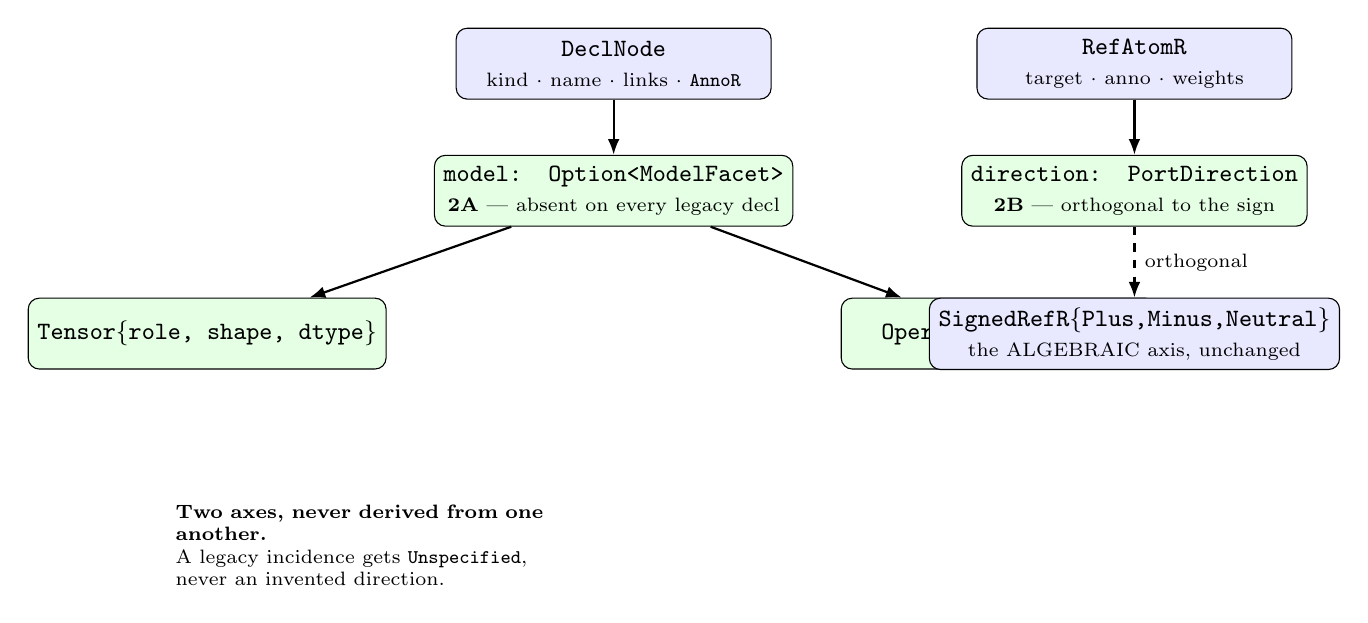
\begin{tikzpicture}[
  node distance=7mm and 12mm,
  box/.style={draw,rounded corners,align=center,minimum width=40mm,minimum height=9mm,font=\small},
  gen/.style={box,fill=blue!9},
  new/.style={box,fill=green!10},
  note/.style={align=left,font=\scriptsize,text width=52mm},
  flow/.style={-{Latex[length=2mm]},thick}
]
\node[gen] (decl) {\texttt{DeclNode}\\\scriptsize kind $\cdot$ name $\cdot$ links $\cdot$ \texttt{AnnoR}};
\node[new,below=of decl] (facet) {\texttt{model: Option<ModelFacet>}\\\scriptsize \textbf{2A} --- absent on every legacy decl};
\node[new,below left=9mm and 6mm of facet] (tensor) {\texttt{Tensor\{role, shape, dtype\}}};
\node[new,below right=9mm and 6mm of facet] (op) {\texttt{Operator\{identity\}}};
\node[gen,right=26mm of decl] (atom) {\texttt{RefAtomR}\\\scriptsize target $\cdot$ anno $\cdot$ weights};
\node[new,below=of atom] (dir) {\texttt{direction: PortDirection}\\\scriptsize \textbf{2B} --- orthogonal to the sign};
\node[gen,below=9mm of dir] (sign) {\texttt{SignedRefR\{Plus,Minus,Neutral\}}\\\scriptsize the ALGEBRAIC axis, unchanged};
\node[note,below=16mm of tensor,xshift=22mm] (rule) {\textbf{Two axes, never derived from one another.}\\A legacy incidence gets \texttt{Unspecified}, never an invented direction.};
\draw[flow] (decl) -- (facet);
\draw[flow] (facet) -- (tensor);
\draw[flow] (facet) -- (op);
\draw[flow] (atom) -- (dir);
\draw[flow,dashed] (dir) -- node[right,font=\scriptsize]{orthogonal} (sign);
\end{tikzpicture}
\end{center}

%======================================================================
\section{Tier 2A --- validated model declaration contract}

\paragraph{Owner.} \texttt{hymeko\_core::ir} for the types, \texttt{ir::coherence} for validation,
\texttt{ir::semantic\_digest} for coverage. No runtime tensor framework enters core: a shape is a
list of extents and a dtype is a closed enum, neither carries data nor arithmetic.

\paragraph{Shape.} Rank-general by construction (\texttt{Vec} of extents, symbolic or static), so
the later CV work is not blocked, while Slice 1 exercises only the small 1-D/2-D MLP shapes.

\paragraph{Acceptance gates.}
\begin{enumerate}\small
\item witness rows 1--6, 9 and 10 become \texttt{CanonicalOwned};
\item an executable model whose tags are replaced by a meaningless word is \textbf{rejected} when a
required typed field is absent, and \textbf{digest-identical} when only the tags differ;
\item a mutation of \texttt{role}, \texttt{shape}, \texttt{dtype} or operator identity moves the
semantic digest --- each with an observation floor proving the field actually changed;
\item serialize $\rightarrow$ parse preserves the typed contract and the digest;
\item the existing corpus decodes unchanged and its v1 digest is byte-identical;
\item a malformed shape, an unknown dtype and an incomplete facet are each rejected for the stated
reason, by a negative control that fails before the fix.
\end{enumerate}

%======================================================================
\section{Tier 2B --- port direction, orthogonal to the sign}

\paragraph{The rule.} \texttt{Plus/Minus/Neutral} is the \emph{algebraic} sign of a signed
hypergraph incidence. It is never read as data-flow direction. \texttt{PortDirection} is a separate
typed axis on \texttt{RefAtomR} with an explicit \texttt{Unspecified} for legacy incidences --- a
legacy edge is never given an invented direction.

\paragraph{Inventory before any signature moves.} Five \texttt{RefAtomR} literal sites in core,
plus the parser/lowering path (\texttt{resolution::resolve}) and the consumers
(\texttt{semantic\_digest}, \texttt{hash\_pass}, \texttt{cbor\_writer::validate},
\texttt{ir::incidence}). Each is enumerated and classified before the field is added.

\paragraph{Acceptance gates.}
\begin{enumerate}\small
\item the witness's data-flow-direction row becomes \texttt{CanonicalOwned};
\item same sign, changed direction $\Rightarrow$ the digest moves;
\item same direction, changed sign $\Rightarrow$ the digest moves, and the two are detected as
\emph{separate} mutations;
\item swapping input and output raises a coherence error;
\item round-trip preserves both axes field-by-field;
\item existing corpus behaviour is explicit: every legacy incidence is \texttt{Unspecified}, asserted.
\end{enumerate}

%======================================================================
\section{Order, and the stop conditions}

2A first, in the smallest coherent slice, with its narrow unit and mutation controls, then the core
integration/serialization/digest gates, then a diff audit. \textbf{2B starts only if 2A is green.}
The full core gate and the canonical MLP witness re-run close the boundary. No WGPU, no Nagare
\texttt{ExecutionPlan}, no CV, no MCU, no dataset campaign, no dependency, no \texttt{CORE.YAML}
schema change beyond the approved-edit ledger entry.

\textbf{Halt immediately} if: a wire-format change cannot be proven compatible; an unknown consumer
appears; a gate passes only vacuously; 2B turns out to be derivable from the sign alone (which would
mean the axes are not orthogonal and the design is wrong); or upstream drift changes the gap.

\paragraph{Rollback.} Every addition is an optional field plus new types. Removing
\texttt{ModelFacet}, the \texttt{direction} field, their digest arms and their tests restores the
prior system exactly; v1 is untouched throughout, so no recorded artifact depends on the change.

\end{document}
